\documentclass[11pt,openany]{article}

\usepackage{mathtools, commath}
% Packages for formatting
\usepackage[margin=1in]{geometry}
\usepackage{fancyhdr}
\usepackage{enumerate}
\usepackage{graphicx}
\usepackage{kotex}
\usepackage{arydshln} % Include this package
\usepackage{bbding}
\usepackage{amsmath}
\usepackage{amsthm}
\usepackage[dvipsnames,table]{xcolor}
\usepackage{amssymb, amsfonts}
\usepackage{wasysym}
\usepackage{footnote}
\usepackage{tablefootnote}
\usepackage{arydshln} % Include this package
% Fonts
\usepackage[T1]{fontenc}
\usepackage[utf8]{inputenc}
\usepackage{newpxtext,newpxmath}
\usepackage{sectsty}

% Define colors
\definecolor{TealBlue1}{HTML}{0077c2}
\definecolor{TealBlue2}{HTML}{00a5e6}
\definecolor{TealBlue3}{HTML}{b3e0ff}
\definecolor{TealBlue4}{HTML}{00293c}
\definecolor{TealBlue5}{HTML}{e6f7ff}

\definecolor{thmcolor}{RGB}{231, 76, 60}
\definecolor{defcolor}{RGB}{52, 152, 219}
\definecolor{lemcolor}{RGB}{155, 89, 182}
\definecolor{corcolor}{RGB}{46, 204, 113}
\definecolor{procolor}{RGB}{241, 196, 15}

\usepackage{color,soul}
\usepackage{soul}
\newcommand{\mathcolorbox}[2]{\colorbox{#1}{$\displaystyle #2$}}
\usepackage{cancel}
\newcommand\crossout[3][black]{\renewcommand\CancelColor{\color{#1}}\cancelto{#2}{#3}}
\newcommand\ncrossout[2][black]{\renewcommand\CancelColor{\color{#1}}\cancel{#2}}

\usepackage{hyperref}
\usepackage{booktabs}

% Chapter formatting
\definecolor{titleTealBlue}{RGB}{0,53,128}
\usepackage{titlesec}
\titleformat{\section}
{\normalfont\sffamily\Large\bfseries\color{titleTealBlue!100!gray}}{\thesection}{1em}{}
\titleformat{\subsection}
{\normalfont\sffamily\large\bfseries\color{titleTealBlue!50!gray}}{\thesubsection}{1em}{}

%Tcolorbox
\usepackage[most]{tcolorbox}
\usepackage{multirow}
\usepackage{multicol}

\usepackage[linesnumbered,ruled]{algorithm2e}
\usepackage{algpseudocode}
\usepackage{setspace}
\SetKwComment{Comment}{/* }{ */}
\SetKwProg{Fn}{Function}{:}{end}
\SetKw{End}{end}
\SetKw{DownTo}{downto}

% Define a new environment for algorithms without line numbers
\newenvironment{algorithm2}[1][]{
	% Save the current state of the algorithm counter
	\newcounter{tempCounter}
	\setcounter{tempCounter}{\value{algocf}}
	% redefine the algorithm numbering (remove prefix)
	\renewcommand{\thealgocf}{}
	\begin{algorithm}
	}{
	\end{algorithm}
	% Restore the algorithm counter state
	\setcounter{algocf}{\value{tempCounter}}
}

\usepackage{adjustbox}
% Header and footer formatting
\pagestyle{fancy}
\fancyhead{}
\fancyhf{}
\rhead{\textcolor{TealBlue2}{\large\textbf{기대수(기초부터 대학원 수학까지 시리즈) 3기}}}%\rule{3cm}{0.4pt}}
\lhead{\textcolor{TealBlue2}{\large\textbf{수학의 즐거움, Enjoying Math}}}
% Define footer
%\newcommand{\footer}[1]{
%\begin{flushright}
%	\vspace{2em}
%	\includegraphics[width=2.5cm]{school_logo.jpg} \\
%	\vspace{1em}
%	\textcolor{TealBlue2}{\small\textbf{#1}}
%\end{flushright}
%}
%\rfoot{\large Department of Information Security, Cryptogrphy and Mathematics, Kookmin Uni.\includegraphics[height=1.5cm]{school_logo.jpg}}
\fancyfoot{}
\fancyfoot[C]{-\thepage-}

\usepackage{tcolorbox}
\tcbset{colback=white, arc=5pt}

\definecolor{axiomcolor}{HTML}{a88bfa}
\definecolor{defcolor}{RGB}{52, 152, 219}
\definecolor{procolor}{RGB}{241, 196, 15}
\definecolor{thmcolor}{RGB}{231, 76, 60}
\definecolor{lemcolor}{RGB}{155, 89, 182}
\definecolor{corcolor}{RGB}{46, 204, 113}
\definecolor{execolor}{RGB}{90, 128, 127}

% Define a new command for the custom tcolorbox
\newcommand{\axiombox}[2][]{%
	\begin{tcolorbox}[colframe=axiomcolor, title={\color{white}\bfseries #1}]
		#2
	\end{tcolorbox}
}

\newcommand{\defbox}[2][]{%
	\begin{tcolorbox}[colframe=defcolor, title={\color{white}\bfseries #1}]
		#2
	\end{tcolorbox}
}

\newcommand{\lembox}[2][]{%
	\begin{tcolorbox}[colframe=lemcolor, title={\color{white}\bfseries #1}]
		#2
	\end{tcolorbox}
}

\newcommand{\probox}[2][]{%
	\begin{tcolorbox}[colframe=procolor, title={\color{white}\bfseries #1}]
		#2
	\end{tcolorbox}
}

\newcommand{\thmbox}[2][]{%
	\begin{tcolorbox}[colframe=thmcolor, title={\color{white}\bfseries #1}]
		#2
	\end{tcolorbox}
}

\newcommand{\corbox}[2][]{%
	\begin{tcolorbox}[colframe=corcolor, title={\color{white}\bfseries #1}]
		#2
	\end{tcolorbox}
}



\usepackage{amsthm}

% Define custom theorem styles
\newtheoremstyle{dotless} % Name of the style
{3pt} % Space above
{3pt} % Space below
{\itshape} % Body font
{} % Indent amount
{\bfseries} % Theorem head font
{} % Punctuation after theorem head
{2.5mm} % Space after theorem head
{} % Theorem head spec

\newtheoremstyle{definitionstyle} % Name of the style
{3pt} % Space above
{3pt} % Space below
{} % Body font
{} % Indent amount
{\bfseries} % Theorem head font
{.} % Punctuation after theorem head
{2.5mm} % Space after theorem head
{} % Theorem head spec

% Applying custom styles
\theoremstyle{dotless}
\newtheorem{theorem}{Theorem} % Theorem environment with section-wise numbering
\newtheorem{proposition}[theorem]{Proposition} % Theorem environment with section-wise numbering
\newtheorem{lemma}[theorem]{Lemma} % Lemma shares the counter with theorem
\newtheorem{corollary}[theorem]{Corollary} % Corollary shares the counter with theorem

\theoremstyle{definitionstyle}
\newtheorem*{observation}{\textcolor{Magenta}{Observation}}
\newtheorem{definition}{Definition} % Definition shares the counter with theorem
\newtheorem{example}{Example} % Example shares the counter with theorem
\newtheorem{exercise}{Exercise} % Example shares the counter with theorem
\newtheorem{remark}{Remark} % Remark shares the counter with theorem
\newtheorem*{note}{Note}

\newtheorem*{definition*}{Definition} % Definition shares the counter with theorem
\newtheorem*{example*}{Example} % Example shares the counter with theorem
\newtheorem*{exercise*}{\textcolor{violet}{Exercise}} % Example shares the counter with theorem
\newtheorem*{remark*}{Remark} % Remark shares the counter with theorem


\usepackage{tikz}
\usepackage{tikz-cd}
\usepackage{tikz-3dplot}
\usepackage{pgfplots}
\pgfplotsset{compat=newest} % Adjust to your version of pgfplots
\def\Circlearrowleft{\ensuremath{%
		\rotatebox[origin=c]{180}{$\circlearrowleft$}}}
\def\Circlearrowright{\ensuremath{%
		\rotatebox[origin=c]{180}{$\circlearrowright$}}}
\def\CircleArrowleft{\ensuremath{%
		\reflectbox{\rotatebox[origin=c]{180}{$\circlearrowleft$}}}}
\def\CircleArrowright{\ensuremath{%
		\reflectbox{\rotatebox[origin=c]{180}{$\circlearrowright$}}}}
\usetikzlibrary{
	3d, % For 3D drawing
	angles,
	arrows,
	arrows.meta,
	backgrounds,
	bending,
	calc,
	decorations.pathmorphing,
	decorations.pathreplacing,
	decorations.markings,
	fit,
	matrix,
	patterns,
	patterns.meta,
	positioning,
	quotes,
	shadows,
	shapes,
	shapes.geometric,
	tikzmark
}
\tikzset{
	% single mid‐path arrow
	mid arrow/.style={
		decoration={
			markings,
			mark=at position 0.5 with {\arrow{Stealth[scale=1.2]}}
		},
		postaction={decorate},
	},
	% style for field arrows
	field arrow/.style={
		-{Stealth[scale=1.0]},
		thick,
		blue!70!black,
	},
}
\newcommand{\ie}{\textnormal{i.e.}}
\newcommand{\rsa}{\mathsf{RSA}}
\newcommand{\rsacrt}{\mathsf{RSA}\textendash\mathsf{CRT}}
\newcommand{\inv}[1]{#1^{-1}}

%New Command
%\newcommand{\set}[1]{\left\{#1\right\}}
\newcommand{\N}{\mathbb{N}}
\newcommand{\Z}{\mathbb{Z}}
\newcommand{\Q}{\mathbb{Q}}
\newcommand{\R}{\mathbb{R}}
\newcommand{\cR}{\mathcal{R}}
\newcommand{\C}{\mathbb{C}}
\newcommand{\F}{\mathbb{F}}
\newcommand{\nbhd}{\mathcal{N}}
\newcommand{\Log}{\operatorname{Log}}
\newcommand{\Arg}{\operatorname{Arg}}
\newcommand{\pv}{\operatorname{P.V.}}

\newcommand{\of}[1]{\left( #1 \right)} 
%\newcommand{\abs}[1]{\left\lvert #1 \right\rvert}
%\newcommand{\norm}[1]{\left\| #1 \right\|}

\newcommand{\sol}{\textcolor{magenta}{\bf Sol}}
\newcommand{\conjugate}[1]{\overline{#1}}

\newcommand{\res}{\operatorname{res}}
\DeclareMathOperator*{\Res}{\operatorname{Res}}

%\renewcommand{\Re}{\operatorname{Re}}
%\renewcommand{\Im}{\operatorname{Im}}

\newcommand{\cyclic}[1]{\langle #1 \rangle}
\newcommand{\uniform}{\overset{\$}{\leftarrow}}
\newcommand{\xmark}{\textcolor{red}{\XSolidBrush}}
\newcommand{\vmark}{\textcolor{green!75!black}{\CheckmarkBold}}

\newcommand{\gen}[1]{\langle #1 \rangle}
\newcommand{\Gen}[1]{\left\langle #1 \right\rangle}

\newcommand{\img}[1]{\text{Img}(#1)}
\newcommand{\Img}[1]{\text{Img}\left(#1\right)}
\newcommand{\preimg}[1]{\text{Img}^{-1}(#1)}
\newcommand{\Preimg}[1]{\text{Img}^{-1}\left(#1\right)}

\newcommand{\relation}{\mathrel{\mathcal{R}}}
\newcommand{\injection}{\rightarrowtail}
\newcommand{\surjection}{\twoheadrightarrow}
\newcommand{\id}{\textnormal{id}}

\newcommand{\eqclass}[1]{\left[#1\right]}

% Define custom colors for O and X
\newcommand{\yes}{\textcolor{blue}{\bf \fullmoon}}
\newcommand{\no}{\textcolor{red}{\bf \texttimes}}

\DeclarePairedDelimiter\ceil{\lceil}{\rceil}
\DeclarePairedDelimiter\floor{\lfloor}{\rfloor}
%\renewcommand{\floor}[#1]{\lfloor #1\rfloor}
%\newcommand{\Floor}[#1]{\left\lfloor #1\right\rfloor}
%\newcommand{\ceil}[#1]{\lceil #1\rceil}
%\newcommand{\Ceil}[#1]{\left\lceil #1\right\rceil}

\newcommand{\topology}{\mathscr{T}}
\newcommand{\sequence}[1]{\langle #1\rangle}

\setstretch{1.25}
\begin{document}
\pagenumbering{arabic}
\begin{center}
	\huge\textbf{Advanced Calculus III}\\
	\vspace{0.5em}
	\large{Ji, Yong-hyeon}\\
%	\large{\ttfamily \url{https://github.com/Hacker-Code-J}}\\
	\vspace{0.5em}
	\normalsize{\today}\\
\end{center}

\noindent 
We cover the following topics in this note.
\begin{itemize}
	\item Limit of a Function
	\item Continuity of a Function
	\item TBA
\end{itemize}
\hrule\vspace{12pt}
What is $\textcolor{red}{0}$ for the set $\textcolor{blue}{S=\set{\frac{1}{n}:n\in\N}}$?
\begin{center}
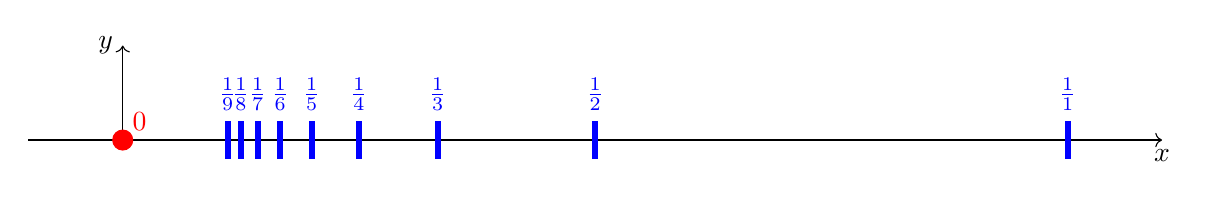
\begin{tikzpicture}[scale=12]
\draw[->] (-0.1, 0) -- (1.1, 0) node[below] {$x$};
\draw[->] (0, -0.01) -- (0, 0.1) node[left] {$y$};
\foreach \n in {1, 2, 3, 4, 5, 6, 7, 8, 9} {
%	\filldraw[blue] ({1/\n}, 0) circle (0.15pt) node[above] {$\frac{1}{\n}$};
\filldraw[blue] ({1/\n-.0025},-.02) rectangle ({1/\n+.0025}, .02);
\filldraw[blue] ({1/\n}, 0) circle (0) node[above=.25cm] {$\frac{1}{\n}$};
}
\filldraw[red] (0, 0) circle (0.3pt) node[above right] {$0$};
\end{tikzpicture}
\end{center}
\begin{note}[Open $\varepsilon$-ball]
	The open $\varepsilon$-ball of $x$ in $S$ is $B_\varepsilon(x):=\set{y\in S:d(x,y)<\varepsilon}$.
\end{note}
\defbox[Limit Point (Metric Space)]{\begin{definition*}
	Let $(X,d)$ be a metric space. Let $S\subseteq X$. A point $p\in X$ is a \textbf{limit point} of $S$ if and only if 
	\[
	\forall\varepsilon>0,\ B_{\varepsilon}(p)\cap (S\setminus\set{p})\neq\varnothing.
	\] That is, \[
	\forall\varepsilon>0,\ \set{x\in S:0< d(x,p)<\varepsilon}\neq\varnothing.
	\]
\end{definition*}}
\begin{center}
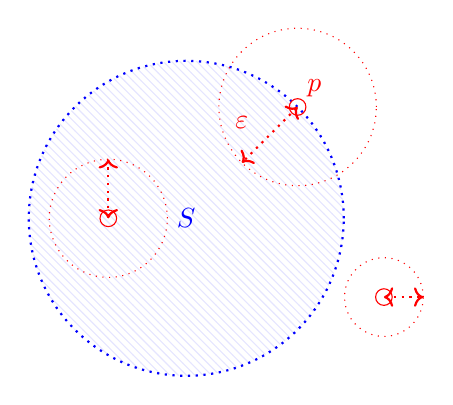
\begin{tikzpicture}[scale=1]
\fill[pattern=north west lines, pattern color=blue!10] (0,0) circle [radius=2];
\draw[dotted, thick, blue] (0,0) circle [radius=2] node[midway, blue] {$S$};

\draw[red] ({sqrt(2)}, {sqrt(2)}) circle (3pt) node[above right] {$p$};
\draw[dotted, red] ({sqrt(2)}, {sqrt(2)}) circle (1cm) node[below] {};
\draw[<->, dotted, thick, red] ({sqrt(2)}, {sqrt(2)}) to ({sqrt(1/2)},{sqrt(1/2)}) node[above=.3cm] {$\varepsilon$};

\draw[red] (-{.7*sqrt(2)}, 0) circle (3pt);
\draw[dotted, red] (-{.7*sqrt(2)}, 0) circle (.75cm);
\draw[<->, dotted, thick, red] (-{.7*sqrt(2)}, 0) to (-{.7*sqrt(2)}, .75);

\begin{scope}[shift={(3.5,-1)}]
	\draw[red] (-{.7*sqrt(2)}, 0) circle (3pt);
	\draw[dotted, red] (-{.7*sqrt(2)}, 0) circle (.5cm);
	\draw[<->, dotted, thick, red] (-{.7*sqrt(2)}, 0) to ({-.7*sqrt(2)+.5}, 0);
\end{scope}
\end{tikzpicture}
\end{center}
\begin{remark*}
	Note that a limit point $p$ may NOT belong to $S$.
\end{remark*}
\begin{note}[Limit Point (Topology)]
	Let $(X,\tau)$ be a topological space. For a subset $S\subseteq X$. A point $p\in X$ is a limit point of $S$ if and only if \[
	\forall U\in\tau\ \text{with}\ p\in U,\ U\cap (S\setminus\set{p})\neq\varnothing.
	\]
\end{note}
\newpage
\begin{example*}
	Let $S=(a,b)\subseteq\R$:
	\begin{center}
	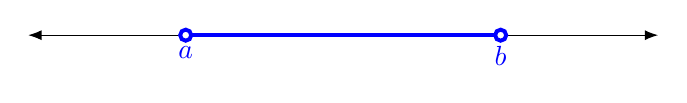
\begin{tikzpicture}
		\draw[Latex-Latex] (-4,0) to (4,0);
		\draw[line width=.5mm, blue] (-2,0) to (2,0);
		\draw[line width=.5mm, blue, fill=white] (-2,0) circle (2pt) node[below] {$a$};
		\draw[line width=.5mm, blue, fill=white] (2,0) circle (2pt) node[below] {$b$};
	\end{tikzpicture}
	\end{center}
\begin{itemize}
	\item Consider $p$ with $p<a$:
	\begin{center}
	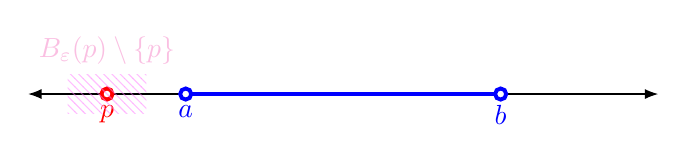
\begin{tikzpicture}
		\draw[Latex-Latex] (-4,0) to (4,0);
		\draw[line width=.5mm, blue] (-2,0) to (2,0);
		\draw[line width=.5mm, blue, fill=white] (-2,0) circle (2pt) node[below] {$a$};
		\draw[line width=.5mm, blue, fill=white] (2,0) circle (2pt) node[below] {$b$};
		\draw[line width=.5mm, red, fill=white] (-3,0) circle (2pt) node[below] {$p$};
		\fill[pattern=north west lines, pattern color=magenta!50, opacity=.5] (-3.5, -.25) rectangle (-2.5, 0.25);
		\node[above=.25cm, magenta!50, opacity=.5] at (-3,0) {$B_\varepsilon(p)\setminus\set{p}$};
%		\draw[decorate, decoration={brace, amplitude=5pt}, thick, color=magenta] (-3, .1) -- (-2.5, .1)
%		node[midway, above=5pt, color=magenta] {\( \varepsilon \)};
	\end{tikzpicture}
	\end{center}
	Let $\varepsilon:=\frac{a-p}{2}>0$. Then $B_\varepsilon(p)\cap (S\setminus\set{p})=\varnothing$. Thus, $p<a$ is NOT a limit point.
	\item Consider $p=a$:
	\begin{center}
	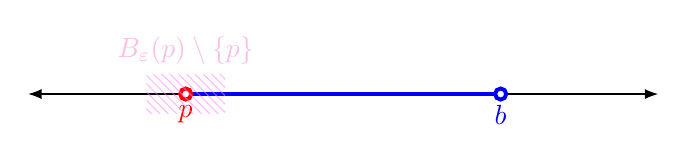
\begin{tikzpicture}
		\draw[Latex-Latex] (-4,0) to (4,0);
		\draw[line width=.5mm, blue] (-2,0) to (2,0);
%		\draw[line width=.5mm, blue, fill=white] (-2,0) circle (2pt) node[below] {$a$};
		\draw[line width=.5mm, blue, fill=white] (2,0) circle (2pt) node[below] {$b$};
		\draw[line width=.5mm, red, fill=white] (-2,0) circle (2pt) node[below] {$p$};
		\fill[pattern=north west lines, pattern color=magenta!50, opacity=.5] (-2.5, -.25) rectangle (-1.5, 0.25);
		\node[above=.25cm, magenta!50, opacity=.5] at (-2,0) {$B_\varepsilon(p)\setminus\set{p}$};
	\end{tikzpicture}
	\end{center}
	Let $\varepsilon>0$. Then $B_\varepsilon(p)\cap (S\setminus\set{p})\neq\varnothing$. Thus, $p=a$ is a limit point of $S=(a,b)$.
\end{itemize}
Hence the set of all limit points of $\intoo{a,b}$ is $\intcc{a,b}$.
\end{example*}
\vfill
\begin{example*}
	Let $S=\set{\frac{1}{n}:n\in\N}$:
	\begin{center}
	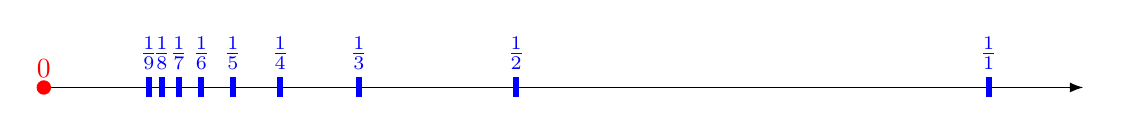
\begin{tikzpicture}[scale=12]
		\draw[-Latex] (0, 0) -- (1.1, 0) node[right] {};
		\foreach \n in {1, 2, 3, 4, 5, 6, 7, 8, 9} {
			%	\filldraw[blue] ({1/\n}, 0) circle (0.15pt) node[above] {$\frac{1}{\n}$};
			\filldraw[blue] ({1/\n-.0025},-.01) rectangle ({1/\n+.0025}, .01);
			\filldraw[blue] ({1/\n}, 0) circle (0) node[above=.1cm] {$\frac{1}{\n}$};
		}
		\filldraw[red] (0, 0) circle (0.2pt) node[above] {$0$};
	\end{tikzpicture}
	\end{center}
	\begin{itemize}
		\item Consider $p=\frac{1}{n}\in S$. No point of $S$ is a limit point.
		\item Consider $p=0$.
		\begin{center}
		\begin{tikzpicture}[scale=12]
			\draw[-Latex] (0, 0) -- (.5, 0) node[right] {};
			\filldraw[blue] ({1/9-.0025},-.01) rectangle ({1/9+.0025}, .01);
			\filldraw[blue] ({1/9}, 0) circle (0) node[above=.1cm] {$\frac{1}{n}$};
			\filldraw[magenta] ({1/5-.0025},-.015) rectangle ({1/5+.0025}, .015);
			\filldraw[magenta] ({1/5}, 0) circle (0) node[above=.15cm] {$\varepsilon$};
%			\foreach \n in {9} {
%				%	\filldraw[blue] ({1/\n}, 0) circle (0.15pt) node[above] {$\frac{1}{\n}$};
%				\filldraw[blue] ({1/\n-.0025},-.01) rectangle ({1/\n+.0025}, .01);
%				\filldraw[blue] ({1/\n}, 0) circle (0) node[above=.1cm] {$\frac{1}{n}$};
%			}
			\filldraw[red] (0, 0) circle (0.2pt) node[above] {$0$};
		\end{tikzpicture}
		\end{center}
		Let $\varepsilon>0$. By Archimedian property, \[
		\exists n\in\N\ \text{such that}\ n>\frac{1}{\varepsilon},
		\] and so $1/n\in B_\varepsilon(0)\cap S$. Thus, $p=0$ is a limit point of $S=\set{1/n:n\in\N}$.
	\end{itemize}
\end{example*}

\newpage

\begin{example*}
Let $S=\Q$.
\begin{itemize}
	\item Consider $p\in\R$. Let $\varepsilon>0$. By density of rationals, \[
	\exists r\in\Q\ \text{such that}\ p<r<p+\varepsilon.
	\] Then $r\in B_\varepsilon(p)\cap S$ with $r\neq p$, \ie, $r$ is a limit points. Thus, all reals are limit points of $\Q$.
\end{itemize}
\end{example*}
%\begin{center}
%\begin{tikzpicture}[scale=3]
%	% Draw the coordinate axes
%%	\draw[->] (-2, 0) -- (4, 0) node[right] {x};
%%	\draw[->] (0, -2) -- (0, 4) node[above] {y};
%	% Define the set of points
%	\foreach \x/\y in {0.5/1, 1.5/0.5, 2/1.5, 2.5/2.2, 1.8/2.5, 1.2/2.3, 0.8/1.8} {
%		\fill[blue] (\x, \y) circle[radius=2pt];
%	}
%	% Highlight the limit point
%	\fill[red] (2, 1) circle[radius=2.5pt] node[below right] {$\alpha$};
%	% Draw the open ball
%	\draw[green!60!black, thick, dashed] (2, 1) circle (1);
%	\node[green!60!black] at (3, 2) {$B_\varepsilon(\alpha)$};
%	% Annotate nearby points in the open ball
%	\foreach \x/\y in {1.5/0.5, 2/1.5, 2.5/2.2} {
%		\draw[->, orange, thick] (\x, \y) -- (2, 1);
%	}
%	
%	% Explanation of other points
%	\node[blue] at (0.5, 0.5) {Other points in the set};
%	\node[red] at (2.8, 0.8) {Limit point $p$};
%\end{tikzpicture}
%\end{center}
\vfill
\defbox[$\star$ Limit of a Function ($\varepsilon-\delta$) $\star$]{\begin{definition*}
	Let $f:X\to\R$ be a function defined on a subset $X(\subseteq\R)$ of a metric space, and let $p\in X$ be a limit point of $X$. We say that $L\in\R$ is the \textbf{limit of the function $f$ as $x$ approaches $p$} if
	\[
	\boxed{\forall\varepsilon>0,\ \exists\delta>0\ \text{such that}\ \forall x\in X,\ 0<\abs[0]{x-p}<\delta\implies\abs[0]{f(x)-L}<\varepsilon}.
	\] We write \[
	\boxed{\lim\limits_{x\to p} f(x)=L}.
	\]
\end{definition*}}
\begin{center}
\begin{minipage}{.49\textwidth}
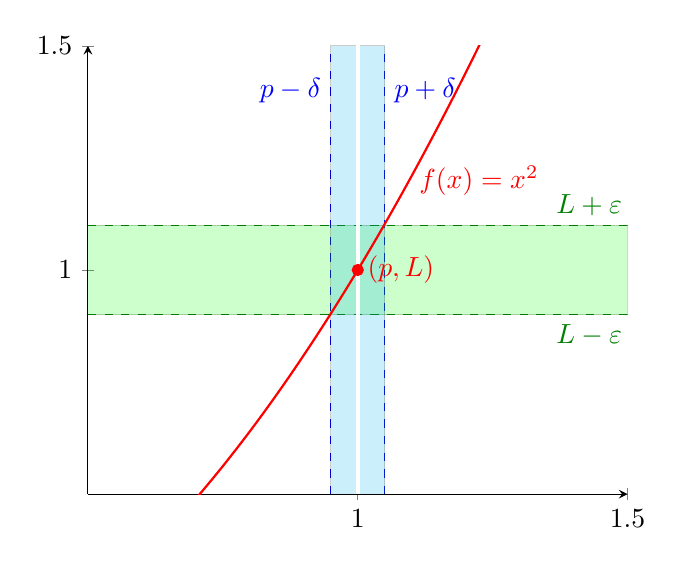
\begin{tikzpicture}
\begin{axis}[
axis lines=middle,
%xlabel={$x$},
%ylabel={$f(x)$},
xmin=0.5, xmax=1.5,
ymin=0.5, ymax=1.5,
xtick={0.5, 1, 1.5},
ytick={0.5, 1, 1.5},
xlabel style={below right},
ylabel style={above left},
legend pos=outer north east,
samples=100
]
% Horizontal epsilon bounds: L-eps and L+eps
\addplot[dashed, green!50!black] coordinates {(0.5, 0.9) (1.5, 0.9)} node[pos=0.85, below right] {$L - \varepsilon$};
\addplot[dashed, green!50!black] coordinates {(0.5, 1.1) (1.5, 1.1)} node[pos=0.85, above right] {$L + \varepsilon$};

% Vertical delta bounds: c-delta and c+delta
\addplot[dashed, blue] coordinates {(0.95, 0.5) (0.95, 1.5)} node[pos=0.9, left] {$p - \delta$};
\addplot[dashed, blue] coordinates {(1.05, 0.5) (1.05, 1.5)} node[pos=0.9, right] {$p + \delta$};

% Shaded area for epsilon bound
\addplot[fill=green, opacity=0.2] coordinates {
	(0.5, 0.9)
	(1.5, 0.9)
	(1.5, 1.1)
	(0.5, 1.1)
	(0.5, 0.9)
};

% Shaded area for delta bound
\addplot[fill=cyan, opacity=0.2] coordinates {
%	(0.9, 0.5)
	(1.05, 0.5)
	(1.05, 1.5)
	(0.95, 1.5)
	(0.95, 0.5)
};


% Shaded area for delta bound
\addplot[fill=white, draw=white] coordinates {
%	(0.9, 0.5)
	(1.0025, 0.5)
	(1.0025, 1.5)
	(0.9975, 1.5)
	(0.9975, 0.5)
};

% Function plot: f(x) = x^2
\addplot[domain=0.5:1.5, thick, red] {x^2} node[midway, right] {$f(x) = x^2$};
% Highlight point (c, L)
\addplot[only marks, mark=*, red] coordinates {(1, 1)} node[below, right] {$(p, L)$};
\end{axis}
\end{tikzpicture}
\end{minipage}\hfill
\begin{minipage}{.49\textwidth}
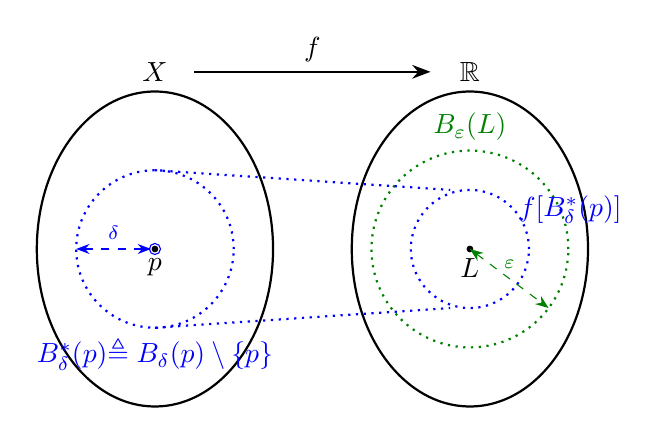
\begin{tikzpicture}[scale=1]
	\draw[thick] (-2,0) ellipse (1.5 and 2);
	\draw[blue, dotted, thick] (-2,0) ellipse (1 and 1);
	\node[below, blue,align=center] at (-2,-1) {$B_\delta^*(p)$$\triangleq B_\delta(p)\setminus\set{p}$};
	\draw[thick] (2,0) ellipse (1.5 and 2);
	\node[green!50!black, above] at (2,1.25) {$B_\varepsilon(L)$};
	\draw[green!50!black, dotted, thick] (2,0) ellipse (1.25 and 1.25);
	\draw[blue, dotted, thick] (2,0) ellipse (.75 and .75);
	\node[blue, right, align=left] at (2.5,.5) {$f[B_\delta^*(p)]$};
	
	% Labels for sets
	\node at (-2, 2.25) {$X$};
	\node at (2, 2.25) {$\R$};
	
	% Draw the arrows representing the function
	\draw[-Stealth, thick] (-1.5, 2.25) -- (1.5,2.25) node[midway, above] {$f$};
	
	%	\node at (2, 1.25) {$f[A]$};
	\draw[blue, dotted, thick] (-2, 1) -- (1.75, .75);
	\draw[blue, dotted, thick] (-2, -1) -- (1.75, -.75);
	
	\filldraw (-2,0) circle (1pt) node[below] {$p$};
	\draw[blue] (-2,0) circle (2pt);
	\filldraw (2,0) circle (1pt) node[below] {$L$};
	%	\draw[|->] (-1.85, 0) -- (1.85, 0);
	
	\draw[>=Stealth, <->, dashed, green!50!black] (2, 0) -- (3,-.75) node[midway, above] {\scriptsize $\varepsilon$};
	\draw[>=Stealth, <->, dashed, blue] (-2.05, 0) -- (-3,0) node[midway, above] {\scriptsize $\delta$};
\end{tikzpicture}
\end{minipage}
\end{center}
%\begin{center}
%\begin{tikzpicture}[scale=1.5]
%	\draw[thick] (-2,0) ellipse (1.5 and 2);
%	\draw[blue, dotted, thick] (-2,0) ellipse (1 and 1);
%	\node[above, blue] at (-2,1) {$B_\delta^*(p)\triangleq B_\delta(p)\setminus\set{p}$};
%	\draw[thick] (2,0) ellipse (1.5 and 2);
%	\node[red, above] at (2,1.25) {$B_\varepsilon(L)$};
%	\draw[red, dotted, thick] (2,0) ellipse (1.25 and 1.25);
%	\draw[blue, dotted, thick] (2,0) ellipse (.75 and .75);
%	\node[blue, right, align=left] at (2.5,.5) {$f[B_\delta^*(p)]$};
%	
%	% Labels for sets
%	\node at (-2, 2.25) {$X$};
%	\node at (2, 2.25) {$\R$};
%	
%	% Draw the arrows representing the function
%	\draw[-Stealth, thick] (-1.5, 2.25) -- (1.5,2.25) node[midway, above] {$f$};
%	
%	%	\node at (2, 1.25) {$f[A]$};
%	\draw[blue, dotted, thick] (-2, 1) -- (1.75, .75);
%	\draw[blue, dotted, thick] (-2, -1) -- (1.75, -.75);
%	
%	\filldraw (-2,0) circle (1pt) node[below] {$p$};
%	\draw[blue] (-2,0) circle (2pt);
%	\filldraw (2,0) circle (1pt) node[below] {$L$};
%%	\draw[|->] (-1.85, 0) -- (1.85, 0);
%	
%	\draw[>=Stealth, <->, dashed, red] (2, 0) -- (3,-.75) node[midway, above] {\scriptsize $\varepsilon$};
%	\draw[>=Stealth, <->, dashed, blue] (-2.05, 0) -- (-3,0) node[midway, above] {\scriptsize $\delta$};
%\end{tikzpicture}
%\end{center}
\begin{remark*}
\[
\lim\limits_{x\to p} f(x)\neq L\iff \exists\varepsilon>0:[\forall\delta>0:\exists x\in X: 0<\abs[0]{x-p}<\delta\ \text{but}\ \abs[0]{f(x)-L}>0].
\]
\end{remark*}
\defbox[Continuity of a Function]{\begin{definition*}
	Let $f:X\to\R$ be a function defined on a subset $X\subseteq\R$ of a metric space, and let $p\in X$. The function $f$ is \textbf{continuous at $p$} if and only if \[
	\lim\limits_{x\to p}f(x)=f(p).
	\] That is, \[
	\forall\varepsilon>0,\ \exists\delta>0\ \text{such that}\ \abs[0]{x-p}<\delta\implies\abs[0]{f(x)-f(p)}<\varepsilon.
	\]
\end{definition*}}
\begin{remark*}[Continuity of a Set]
	The function $f$ is continuous on subset $S\subseteq X$ if it it continuous at every point $p\in S$.
\end{remark*}
\begin{remark*}[Continuity in a Topological Space]
	Let $(X,\tau_X)$ and $(Y,\tau_Y)$ are topological spaces. $f:X\to Y$ is \textbf{continuous} if and only if $$U_Y\in\tau_Y\implies f^{-1}[U_Y]\in\tau_X,$$ where $f^{-1}[U_Y]=\set{x\in X:f(x)\in U_Y}$ is the preimage of $U_Y$ under $f$.
\end{remark*}
\vfill
\begin{note}
	$[p\Rightarrow(q\Rightarrow r)]\equiv [p\Rightarrow(\lnot q\lor r)]\equiv[\lnot p\lor (\lnot q\lor r)]\equiv [\lnot (p\land q)\lor r]\equiv [(p\land q)\Rightarrow r]$.
\end{note}
\thmbox[Limit of Function by Convergent Sequences]{\begin{theorem*}
Let $f:X\to\R$ be a function defined on a subset $\varnothing\neq X\subseteq\R$ of a topological space, and let $p$ is a limit point of $X$. Then \[
\lim\limits_{x\to p}f(x)=L\iff\left[\forall\set{x_n}\subseteq X\setminus\set{p},\left(\lim\limits_{n\to\infty}x_n=p\implies\lim\limits_{n\to\infty}f(x_n)=L\right)\right].
\]
\end{theorem*}}
\begin{center}
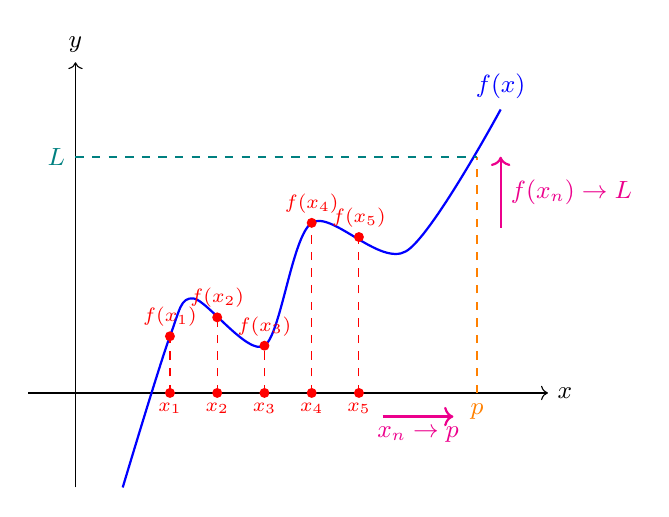
\begin{tikzpicture}[scale=1.2, every node/.style={font=\small}]
	% Axes
	\draw[->] (-0.5, 0) -- (5, 0) node[right] {$x$};
	\draw[->] (0, -1) -- (0, 3.5) node[above] {$y$};
	
	\begin{scope}[shift={(-.5,3)}]
		\draw[color=blue,thick,smooth] plot coordinates {(1,-4) (1.5,-2.4) (1.75,-2) (2.5,-2.5) (3,-1.2) (4,-1.5) (5,0)} node[above] {$f(x)$};
	\end{scope}
	
	% Points and labels for the sequence x_n
	\foreach \n/\x/\y in {1/1/.6, 2/1.5/.8, 3/2/.5, 4/2.5/1.8, 5/3/1.65}
	{
		\fill[red] (\x, \y) circle (1.5pt) node[above] {\scriptsize $f(x_{\n})$};
		\fill[red] (\x, 0) circle (1.5pt) node[below] {\scriptsize $x_{\n}$};
		\draw[red, dashed] (\x, 0) -- (\x, \y);
	}

	% Converging sequence x_n -> a
	\draw[magenta, ->, thick] (3.25, -0.25) -- (4, -0.25) node[midway, below] {$x_n \to p$};
	
	% Converging sequence f(x_n) -> L
	\draw[magenta, ->, thick] (4.5, 1.75) -- (4.5, 2.5) node[midway, right] {$f(x_n) \to L$};
	
	% Labels for a and L
	\draw[dashed, thick, orange] (4.25, 0) node[below] {$p$} -- (4.25, 2.5);
	\draw[dashed, thick, teal] (0, 2.5) node[left] {$L$} -- (4.25, 2.5);
	
\end{tikzpicture}
\end{center}
%\begin{tikzpicture}[scale=1.5]
%	% Axes
%	\draw[->] (-1, 0) -- (5, 0) node[right] {\(x\)};
%	\draw[->] (0, -1) -- (0, 4) node[above] {\(y\)};
%	
%	% Function curve
%	\draw[domain=0.5:4, smooth, variable=\x, thick] plot ({\x}, {2 + 0.5*sin(3*\x r)});
%	\node[below right] at (4, 3) {\(f(x)\)};
%	
%	% Limit point
%	\node[below] at (2, 0) {\(p\)};
%	\node[left] at (0, 2.5) {\(L\)};
%	\draw[dashed] (2, 0) -- (2, 2.5);
%	\draw[dashed] (0, 2.5) -- (2, 2.5);
%	
%	% Sequence points
%	\foreach \i in {1, 2, 3, 4} {
%		\pgfmathsetmacro{\xn}{2 - 1/\i}
%		\pgfmathsetmacro{\yn}{2.5 + 0.5*sin(3*\xn r)}
%		\draw[fill=blue] (\xn, \yn) circle (1pt);
%		\draw[dashed, blue] (\xn, \yn) -- (\xn, 0);
%		\node[below] at (\xn, 0) {\(x_{\i}\)};
%	}
%	
%	% Sequence convergence
%	\draw[->, thick, red] (1.2, 3.5) -- (2, 2.5) node[above left] {\(f(x_n) \to L\)};
%\end{tikzpicture}
\begin{proof}
\begin{itemize}
	\item[($\Rightarrow$)] Suppose that $\lim\limits_{x\to p}f(x)=L$. Let $\set{x_n}\subseteq X\setminus\set{p}$ be a sequence, and let $\lim\limits_{n\to\infty}x_n=p$. We NTS that \[
	\lim\limits_{n\to\infty}f(x_n)=L,\quad\ie,\color{blue}\quad\forall\varepsilon>0:\exists N\in\N:n\geq N\Rightarrow\abs[0]{f(x_n)-L}<\varepsilon.
	\] \textcolor{blue}{Let $\varepsilon>0$}. Since $\lim\limits_{x\to p}f(x)=L$, we know \begin{equation*}
		\exists\delta>0\ \text{such that}\ 0<\abs[0]{x-p}<\delta\implies\abs[0]{f(x)-L}<\varepsilon.\tag{*}
	\end{equation*} Since $\lim\limits_{n\to\infty}x_n=p$, we obtain \[
	\textcolor{blue}{\exists N\in\N}\ \text{such that}\ n\geq N\implies\abs[0]{x_n-p}<\delta.
	\] Thus, \textcolor{blue}{if $n\geq N$ then}, \begin{align*}
		\abs[0]{x_n-p}<\delta&\implies 0<\abs[0]{x_n-p}<\delta\quad\because x_n\neq p \\
		&\implies\textcolor{blue}{\abs[0]{f(x_n)-L}<\varepsilon}\quad\text{by (*)}
	\end{align*} Thus, $\lim\limits_{n\to\infty}f(x_n)=L$.
	\item[($\Leftarrow$)] Let the RHS holds. Assume, for the contradiction, that $\lim\limits_{x\to p} f(x)\neq L$, \ie, \[
	\textcolor{green!50!black}{\exists\varepsilon>0}:\forall\delta>0:\exists x_\delta\in X:0<\abs[0]{x_\delta-p}<\delta\ \text{but}\ \textcolor{magenta}{\abs[0]{f(x_\delta)-L}\geq\varepsilon}.
	\] Take $\delta=1/n$ for $n\in\N$. Then \[
	\exists x_n\in X\ \text{such that}\ 0<\abs[0]{x_n-p}<\delta\ \text{but}\ \abs[0]{f(x_n)-L}\geq \varepsilon.
	\] \textcolor{gray!50}{\st{(Axiom of Countable Choice)}}\ This means that \[
	\forall n\in\N:\exists\set{x_n}\subseteq X\setminus\set{p}\ \text{such that}\ 0<\abs[0]{x_n-p}<\frac{1}{n}\ \text{but}\ \textcolor{magenta}{\abs[0]{f(x_n)-L}\geq \varepsilon}.
	\] By Squeeze Theorem, we have $\lim\limits_{n\to\infty}x_n=p$ since $0<\abs[0]{x_n-p}<1/n$. Since the RHS holds, we obtain $\lim\limits_{n\to\infty}f(x_n)=L$. Then, for some $\textcolor{green!50!black}{\varepsilon>0}$, \[
	\exists N\in\N\ \text{such that}\ n\geq N\implies\textcolor{magenta}{\abs{f(x_n)-L}<\varepsilon}\ \text{\Large\lightning}.
	\] Hence it is proved.
\end{itemize}
\end{proof}
\corbox[Continuity of Function by Convergent Sequences]{\begin{corollary*}
Let $f:X\to\R$ be a function defined on a subset $\varnothing\neq X\subseteq\R$ of a topological space, and let $p$ is a limit point of $X$. Then \[
\lim\limits_{x\to p}f(x)=f(p)\iff\left[\forall\set{x_n}\subseteq X,\left(\lim\limits_{n\to\infty}x_n=p\implies\lim\limits_{n\to\infty}f(x_n)=f(p)\right)\right].
\]
\end{corollary*}}
\vfill
\thmbox[Squeeze Theorem; Sandwich Theorem]{\begin{theorem*}
	Let \begin{enumerate}[(i)]
		\item $\lim\limits_{n\to\infty}a_n=L=\lim\limits_{n\to\infty}b_n$;
		\item $\exists n_0\in\N$ such that $a_n\leq c_n\leq b_n$ for all $n\geq n_0$.
	\end{enumerate} Then $
	\lim\limits_{n\to\infty}c_n=L.$
\end{theorem*}}
\begin{center}
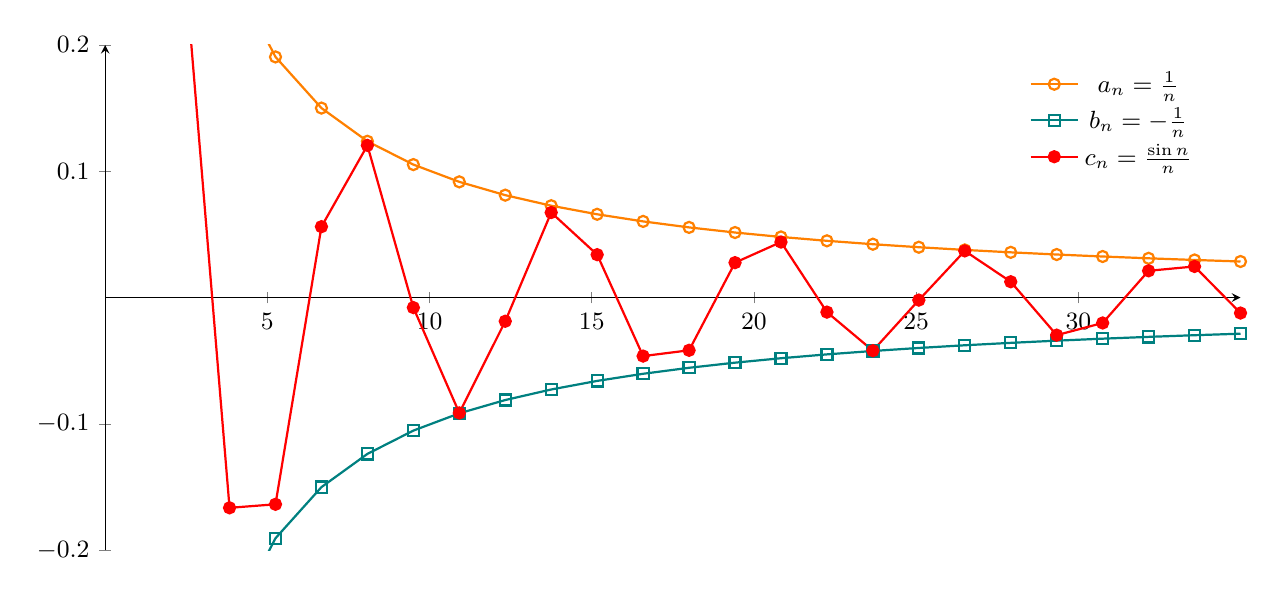
\begin{tikzpicture}
	\begin{axis}[
		width=16cm, height=8cm, % Size of the plot
		axis lines=middle,
%		xlabel={$n$},
%		ylabel={$a_n, b_n, c_n$},
		xmin=0, xmax=35, % n range
		ymin=-0.2, ymax=0.2, % y range
		xtick={0,5,10,15,20,25,30}, % n ticks
		ytick={-0.2,-0.1,0,0.1,0.2}, % y ticks
		legend style={draw=none, fill=none, font=\small},
		legend pos=north east,
		every axis x label/.style={at={(current axis.right of origin)}, anchor=north},
		every axis y label/.style={at={(current axis.above origin)}, anchor=east},
		tick label style={font=\small}
		]
		
		% Plot a_n = 1/n
		\addplot[domain=1:35, thick, orange, mark=o] {1/x};
		\addlegendentry{$a_n = \frac{1}{n}$}
		
		% Plot b_n = -1/n
		\addplot[domain=1:35, thick, teal, mark=square] {-(1/x)};
		\addlegendentry{$b_n = -\frac{1}{n}$}
		
		% Plot c_n = sin(n)/n
		\addplot[domain=1:35, thick, red, mark=*] {sin(deg(x))/x};
		\addlegendentry{$c_n = \frac{\sin n}{n}$}
	\end{axis}
\end{tikzpicture}
\end{center}
\begin{proof}
\textcolor{blue}{Let $\varepsilon>0$}. Since $\lim\limits_{n\to\infty}a_n=L$ and $\lim\limits_{n\to\infty}a_n=L$, we have \begin{align*}
\exists n_1\in\N\ \text{such that}\ n\geq n_1&\implies L-\varepsilon<a_n\textcolor{gray}{<L+\varepsilon},\\
\exists n_2\in\N\ \text{such that}\ n\geq n_2&\implies \textcolor{gray}{L-\varepsilon}<b_n<L+\varepsilon.
\end{align*} Let \textcolor{blue}{$N:=\max\set{n_0,n_1,n_2}$}. \textcolor{blue}{If $n\geq N$ then} \[
L-\varepsilon<a_n\leq c_n\leq b_n<L_+\varepsilon,
\] and so \textcolor{blue}{$\abs[0]{c_n-L}<\varepsilon$}.
\end{proof}
%\newpage
%\begin{example*} Prove that \[
%\lim\limits_{n\to\infty}n^{\frac{1}{n}} = 1.	
%\]
%\begin{center}
%\begin{tikzpicture}
%\begin{axis}[
%	width=12cm, height=8cm, % Plot size
%	axis lines=middle,
%%	xlabel={$n$},
%%	ylabel={$a_n = n^{1/n}$},
%	xmin=1, xmax=30, % Set x-axis range
%	ymin=0.9, ymax=1.5, % Set y-axis range
%	xtick={0,5,10,15,20,25,30}, % Custom x-ticks
%	ytick={0.9,1,1.1,1.2}, % Custom y-ticks
%	legend style={draw=none, fill=none, font=\small},
%	legend pos=north east,
%	every axis x label/.style={at={(current axis.right of origin)}, anchor=south},
%	every axis y label/.style={at={(current axis.above origin)}, anchor=west},
%	tick label style={font=\small}
%	]
%	% Plot a_n = n^(1/n)
%	\addplot[domain=1:30, thick, blue, mark=*] {x^(1/x)};
%	\addlegendentry{$x_n = n^{1/n}$}
%	
%	% Plot y = 1 (limit line)
%	\addplot[dashed, red] coordinates {(1,1) (30,1)};
%	\addlegendentry{$L = 1$}
%\end{axis}
%\end{tikzpicture}
%\end{center}
%\begin{proof}[\sol]
%	Let $x_n=n^{1/n}$ and $x_n=1+a_n$. Then
%\end{proof}
%\begin{tikzpicture}
%\ \\	\begin{axis}[
%		width=12cm, height=8cm, % Set plot size
%		axis lines=middle,
%		xlabel={$n$},
%		ylabel={$a_n, b_n$},
%		xmin=1, xmax=20, % Set x-axis range
%		ymin=-2, ymax=2, % Set y-axis range
%		xtick={1,5,10,15,20}, % Custom x-ticks
%		ytick={0.9,1,1.1,1.2}, % Custom y-ticks
%		legend style={draw=none, fill=none, font=\small},
%		legend pos=south east,
%		every axis x label/.style={at={(current axis.right of origin)}, anchor=north},
%		every axis y label/.style={at={(current axis.above origin)}, anchor=east},
%		tick label style={font=\small}
%		]
%		% Plot b_n = sqrt(2/(n-1))
%		\addplot[domain=2:20, thick, red, mark=o] {sqrt(2/(x-1))};
%		\addlegendentry{$b_n = \sqrt{\frac{2}{n-1}}$}
%		
%		% Plot a_n = 1 + b_n
%		\addplot[domain=2:20, thick, blue, mark=*] {1 + sqrt(2/(x-1))};
%		\addlegendentry{$a_n = 1 + b_n$}
%		
%		% Plot y = 1 (limit line for a_n)
%		\addplot[dashed, black] coordinates {(1,1) (20,1)};
%		\addlegendentry{$L = 1$}
%		
%		% Annotate
%		\node[anchor=south] at (axis cs:15,1.15) {As $n \to \infty, \ b_n \to 0$ and $a_n \to 1$};
%	\end{axis}
%\end{tikzpicture}
%\end{example*}

\newpage
\thmbox[Monotone Convergence Theorem (MCT)]{\begin{theorem*}
	TBA
\end{theorem*}}
\begin{proof}
	TBA
\end{proof}

\thmbox[Nested Interval Property (NIP)]{\begin{theorem*}
	TBA
\end{theorem*}}
\begin{proof}
	TBA
\end{proof}

%\begin{tikzpicture}
%	
%	% Create a pgfplots environment
%	\begin{axis}[
%		axis lines=middle,
%		xlabel={$x$},
%		ylabel={$f(x)$},
%		xmin=0, xmax=1.5,
%		ymin=0, ymax=2.25,
%		width=12cm,
%		height=8cm,
%		grid=both,
%		legend style={font=\small},
%		legend pos=north west,
%		samples=100,
%		domain=0:1.5
%		]
%		
%		% Continuous function f(x)
%		\addplot[line width=.5mm, blue, domain=0:1.5] {x^2} 
%		node[pos=0.8, midway, left=2cm] {\textcolor{blue}{$f(x) = x^2$}};
%		
%		% Horizontal dashed line for limit L
%		\addplot[red, dashed, line width=.5mm] coordinates {(0,2) (1.5,2)} 
%		node[pos=0.9, above] {\textcolor{red}{}};
%		\addplot[red, dashed, line width=.5mm] coordinates {({sqrt(2)},0) ({sqrt(2)},2)};
%		
%		% Point p (limit point)
%		\addplot[mark=*, mark options={red}, only marks] coordinates {({sqrt(2)},2)} 
%		node[below] {\textcolor{red}{}};
%		
%		% Sequence points approaching p
%		\addplot[line width = .75mm, mark=*, teal, opacity=0.75] coordinates {(0,0) (.2,{.2^2}) (.4,{.4^2}) (.9,{.9^2}) ({sqrt(2)},2)}
%		node[pos=0.1, below right] {\textcolor{teal}{$\set{x_n,f(x_n)}$}};
%%		
%%		% Annotate sequence x_n -> p
%%		\draw[->, thick, orange] (axis cs:0.8,0) -- (axis cs:1,0) 
%%		node[midway, below] {\textcolor{orange}{$x_n \to p$}};
%%		
%%		% Annotate f(x_n) -> L
%%		\draw[->, thick, orange] (axis cs:0.99,0.9801) -- (axis cs:1,1) 
%%		node[midway, right] {\textcolor{orange}{$f(x_n) \to L$}};
%%		
%%		% Neighborhood of p
%%		\draw[<->, thick, red] (axis cs:0.85,-0.1) -- (axis cs:1.15,-0.1)
%%		node[midway, below] {\textcolor{red}{$\delta$}};
%		
%		% Legend
%%		\legend{
%%			$f(x)$ (continuous),
%%			Limit $L$,
%%			Limit point $p$,
%%			Sequence points $\{x_n\}$
%%		}
%		
%	\end{axis}
%	
%\end{tikzpicture}


\vfill

\begin{thebibliography}{9}
	\bibitem{advanced_calc_e}
	수학의 즐거움, Enjoying Math. ``수학 공부, 기초부터 대학원 수학까지, 10. 해석학 개론 (e) 엡실론-델타와 수열의 수렴성'' YouTube Video, 25:57. Published 
	September 29, 2019. URL: \url{https://youtu.be/2Ml3G_Duffk?si=qo-CVgW3Ukd4ADRL}.
	\bibitem{advanced_calc_f}
	수학의 즐거움, Enjoying Math. ``수학 공부, 기초부터 대학원 수학까지, 11. 해석학 개론 (f) MCT and NIP'' YouTube Video, 20:17. Published 
	October 1, 2019. URL: \url{https://youtu.be/YdnBQaY5eDk?si=BNe0Ue4iq2P9Fxsd}.
%	\bibitem{advanced_calc_g}
%	수학의 즐거움, Enjoying Math. ``수학 공부, 기초부터 대학원 수학까지, 12. 해석학 개론 (g) Limsup, Liminf'' YouTube Video, 34:31. Published 
%	October 2, 2019. URL: \url{https://youtu.be/4Q1cm3VQPUE?si=phAhKwnOxdnRAiRR}.
\end{thebibliography}
%\newpage
%\appendix
%\section{Complement of Family}
%\begin{note}
%	\[
%	\left(\bigcup_{i\in\Lambda}E_i\right)^C=
%	\bigcap_{i\in\Lambda}\left(E_i\right)^C
%	\]
%	\begin{proof}
%		content...
%	\end{proof}
%\end{note}
\end{document}
